\documentclass[dvips, lscape]{foils}
%\documentclass[dvips, french]{slides}
\textwidth 18.5cm
\textheight 25cm 
\topmargin -1cm 
\oddsidemargin  -1cm 
\evensidemargin  -1cm

% Maths
\usepackage{amsfonts, amsmath, amssymb, url}

\newcommand{\coefbin}[2]{\left( 
    \begin{array}{c} #1 \\ #2 \end{array} 
  \right)}
\newcommand{\bbullet}{\bullet\bullet}
\newcommand{\bbbullet}{\bbullet\bullet}
\newcommand{\bbbbullet}{\bbbullet\bullet}
\newcommand{\Bcal}{\mathcal{B}}
\newcommand{\Ccal}{\mathcal{C}}
\newcommand{\Dcal}{\mathcal{D}}
\newcommand{\Ecal}{\mathcal{E}}
\newcommand{\Gcal}{\mathcal{G}}
\newcommand{\Mcal}{\mathcal{M}}
\newcommand{\Ncal}{\mathcal{N}}
\newcommand{\Pcal}{\mathcal{P}}
\newcommand{\Qcal}{\mathcal{Q}}
\newcommand{\Rcal}{\mathcal{R}}
\newcommand{\Hcal}{\mathcal{H}}
\newcommand{\Jcal}{\mathcal{J}}
\newcommand{\Lcal}{\mathcal{L}}
\newcommand{\Tcal}{\mathcal{T}}
\newcommand{\Ucal}{\mathcal{U}}
\newcommand{\Xcal}{\mathcal{X}}
\newcommand{\Zcal}{\mathcal{Z}}
\newcommand{\e}{\text{e}}
\newcommand{\etabar}{\overline{\eta}}
\newcommand{\pibar}{\overline{\pi}}
\newcommand{\alphabf}{\mbox{\mathversion{bold}{$\alpha$}}}
\newcommand{\betabf}{\mbox{\mathversion{bold}{$\beta$}}}
\newcommand{\gammabf}{\mbox{\mathversion{bold}{$\gamma$}}}
\newcommand{\mubf}{\mbox{\mathversion{bold}{$\mu$}}}
\newcommand{\Pibf}{\mbox{\mathversion{bold}{$\Pi$}}}
\newcommand{\psibf}{\mbox{\mathversion{bold}{$\psi$}}}
\newcommand{\Sigmabf}{\mbox{\mathversion{bold}{$\Sigma$}}}
\newcommand{\taubf}{\mbox{\mathversion{bold}{$\tau$}}}
\newcommand{\thetabf}{\mbox{\mathversion{bold}{$\theta$}}}
\newcommand{\Abf}{{\bf A}}
\newcommand{\Ebf}{{\bf E}}
\newcommand{\Hbf}{{\bf H}}
\newcommand{\Ibf}{{\bf I}}
\newcommand{\Obf}{{\bf 0}}
\newcommand{\Sbf}{{\bf S}}
\newcommand{\mbf}{{\bf m}}
\newcommand{\ubf}{{\bf u}}
\newcommand{\vbf}{{\bf v}}
\newcommand{\xbf}{{\bf x}}
\newcommand{\Xbf}{{\bf X}}
\newcommand{\Esp}{{\mathbb E}}
\newcommand{\Corr}{{\mathbb C}\mbox{orr}}
\newcommand{\Nm}{N(\mbf)}
\newcommand{\mum}{\mu(\mbf)}
\newcommand{\obs}{\text{obs}}
\newcommand{\ERMG}{\text{EMRG}}
\newcommand{\Ibb}{{\mathbb I}}
\newcommand{\Omegas}{\underset{s}{\Omega}}
\newcommand{\Var}{{\mathbb V}}
\newcommand{\Rbb}{\mathbb{R}}
\newcommand{\Vsf}{\mathsf{V}}
\newcommand{\Starsf}{\mathsf{*}}

% Motifs
\newcommand{\Vmotif}{\includegraphics[width=1.3cm]{../Figures/vmotif.eps}}
\newcommand{\trianglemotif}{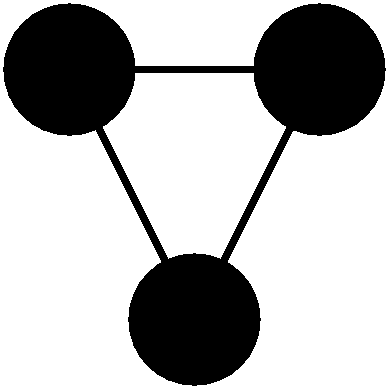
\includegraphics[width=1.3cm]{../Figures/trianglemotif.eps}}
\newcommand{\starmotif}{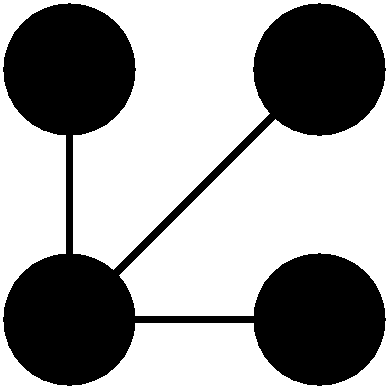
\includegraphics[width=1.3cm]{../Figures/starmotif.eps}}
\newcommand{\chainmotif}{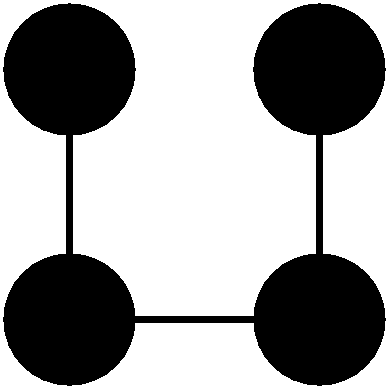
\includegraphics[width=1.3cm]{../Figures/chainmotif.eps}}
\newcommand{\squaremotif}{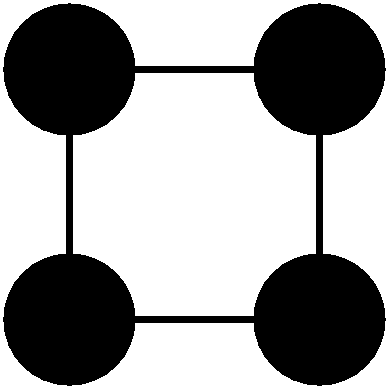
\includegraphics[width=1.3cm]{../Figures/squaremotif.eps}}
\newcommand{\whisker}{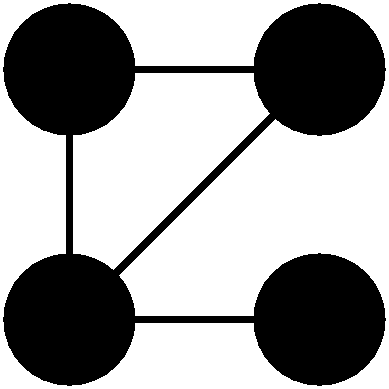
\includegraphics[width=1.3cm]{../Figures/whisker.eps}}
\newcommand{\halfclique}{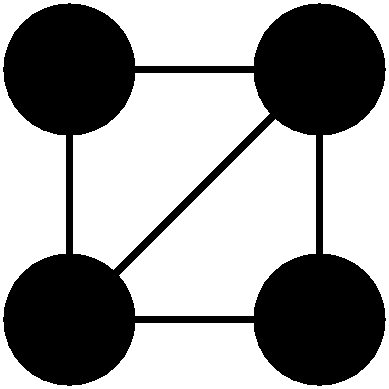
\includegraphics[width=1.3cm]{../Figures/halfclique.eps}}
\newcommand{\clique}{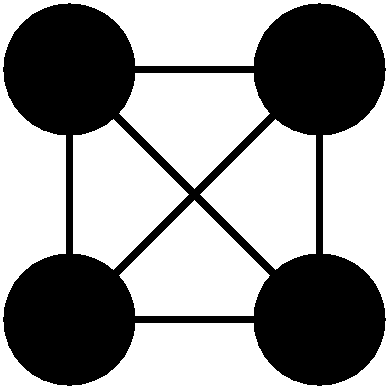
\includegraphics[width=1.3cm]{../Figures/clique.eps}}

% Couleur et graphiques
\usepackage{color}
\usepackage{graphics}
\usepackage{epsfig} 
\usepackage{pstcol}

% Texte
\usepackage{lscape}
\usepackage{../../../../Latex/fancyheadings, rotating, enumerate}
%\usepackage[french]{babel}
\usepackage[latin1]{inputenc}
%\definecolor{darkgreen}{cmyk}{0.5, 0, 0.5, 0.5}
\definecolor{green}{cmyk}{0.5, 0, 0.5, 0.5}
\definecolor{orange}{cmyk}{0, 0.6, 0.8, 0}
\definecolor{jaune}{cmyk}{0, 0.5, 0.5, 0}
\newcommand{\textblue}[1]{\textcolor{blue}{#1}}
\newcommand{\textred}[1]{\textcolor{red}{#1}}
\newcommand{\textgreen}[1]{\textcolor{green}{ #1}}
\newcommand{\textlightgreen}[1]{\textcolor{green}{#1}}
%\newcommand{\textgreen}[1]{\textcolor{darkgreen}{#1}}
\newcommand{\textorange}[1]{\textcolor{orange}{#1}}
\newcommand{\textyellow}[1]{\textcolor{yellow}{#1}}
\newcommand{\emphase}[1]{\textblue{#1}}
\newcommand{\refer}[1]{\textgreen{\sl #1}}

% Sections
%\newcommand{\chapter}[1]{\centerline{\LARGE \textblue{#1}}}
% \newcommand{\section}[1]{\centerline{\Large \textblue{#1}}}
% \newcommand{\subsection}[1]{\noindent{\Large \textblue{#1}}}
% \newcommand{\subsubsection}[1]{\noindent{\large \textblue{#1}}}
% \newcommand{\paragraph}[1]{\noindent {\textblue{#1}}}
% Sectionsred
\newcommand{\chapter}[1]{
  \addtocounter{chapter}{1}
  \setcounter{section}{0}
  \setcounter{subsection}{0}
  {\centerline{\LARGE \textblue{\arabic{chapter} - #1}}}
%  {\centerline{\LARGE \textblue{#1}}}
  }
\newcommand{\section}[1]{
  \addtocounter{section}{1}
  \setcounter{subsection}{0}
  {\centerline{\Large \textblue{\arabic{chapter}.\arabic{section} - #1}}}
%  {\centerline{\Large \textblue{#1}}}
  }
\newcommand{\subsection}[1]{
  \addtocounter{subsection}{1}
%  {\noindent{\large \textblue{\arabic{chapter}.\arabic{section}.\arabic{subsection} - #1}}}
  {\noindent{\large \textblue{#1}}}
  }
\newcommand{\paragraph}[1]{\noindent{\textblue{#1}}}

%%%%%%%%%%%%%%%%%%%%%%%%%%%%%%%%%%%%%%%%%%%%%%%%%%%%%%%%%%%%%%%%%%%%%%
%%%%%%%%%%%%%%%%%%%%%%%%%%%%%%%%%%%%%%%%%%%%%%%%%%%%%%%%%%%%%%%%%%%%%%
%%%%%%%%%%%%%%%%%%%%%%%%%%%%%%%%%%%%%%%%%%%%%%%%%%%%%%%%%%%%%%%%%%%%%%
%%%%%%%%%%%%%%%%%%%%%%%%%%%%%%%%%%%%%%%%%%%%%%%%%%%%%%%%%%%%%%%%%%%%%%
\begin{document}
%%%%%%%%%%%%%%%%%%%%%%%%%%%%%%%%%%%%%%%%%%%%%%%%%%%%%%%%%%%%%%%%%%%%%%
%%%%%%%%%%%%%%%%%%%%%%%%%%%%%%%%%%%%%%%%%%%%%%%%%%%%%%%%%%%%%%%%%%%%%%
%%%%%%%%%%%%%%%%%%%%%%%%%%%%%%%%%%%%%%%%%%%%%%%%%%%%%%%%%%%%%%%%%%%%%%
%%%%%%%%%%%%%%%%%%%%%%%%%%%%%%%%%%%%%%%%%%%%%%%%%%%%%%%%%%%%%%%%%%%%%%
\landscape
\newcounter{chapter}
\newcounter{section}
\newcounter{subsection}
\setcounter{chapter}{0}
\headrulewidth 0pt 
\pagestyle{fancy} 
\cfoot{}
\rfoot{\begin{rotate}{90}{
      \hspace{1cm} \tiny S. Robin: Assessing the exceptionality of
      network motifs  
      }\end{rotate}}
\rhead{\begin{rotate}{90}{
      \hspace{-.5cm} \tiny \thepage
      }\end{rotate}}

%%%%%%%%%%%%%%%%%%%%%%%%%%%%%%%%%%%%%%%%%%%%%%%%%%%%%%%%%%%%%%%%%%%%%%
%%%%%%%%%%%%%%%%%%%%%%%%%%%%%%%%%%%%%%%%%%%%%%%%%%%%%%%%%%%%%%%%%%%%%%
\begin{center}
  \textblue{\LARGE Assessing the exceptionality of network motifs}
  
  \vspace{2cm}
  \textblue{\large J.-J. Daudin, M. Koskas, F. Picard,
  \underline{S. Robin}, S. Schbath} \\
%   ~\\
%   $(^*)$ UMR AgroParisTech / INRA, Paris, \\
%     Math�matique et Informatique Appliqu�es \\
%   \url{www.inapg.inra.fr/ens_rech/maths/} \\
%   ~\\~\\
  \vspace{2cm}
  {Statistics for Biological Sequences group} \\
  (Evry + Jouy en Josas + Paris) \\
  \url{genome.jouy.inra.fr/ssb/}
  ~\\~\\
\end{center}

\paragraph{Research report:} \\
\centerline{\url{genome.jouy.inra.fr/ssb/preprint/SSB-RR-1.netmotifs.pdf}}

%%%%%%%%%%%%%%%%%%%%%%%%%%%%%%%%%%%%%%%%%%%%%%%%%%%%%%%%%%%%%%%%%%%%%
%%%%%%%%%%%%%%%%%%%%%%%%%%%%%%%%%%%%%%%%%%%%%%%%%%%%%%%%%%%%%%%%%%%%%
\newpage
\chapter{Network motifs}
%%%%%%%%%%%%%%%%%%%%%%%%%%%%%%%%%%%%%%%%%%%%%%%%%%%%%%%%%%%%%%%%%%%%%
%%%%%%%%%%%%%%%%%%%%%%%%%%%%%%%%%%%%%%%%%%%%%%%%%%%%%%%%%%%%%%%%%%%%%

%%%%%%%%%%%%%%%%%%%%%%%%%%%%%%%%%%%%%%%%%%%%%%%%%%%%%%%%%%%%%%%%%%%%%
\bigskip
\section{Analysing biological networks}
%%%%%%%%%%%%%%%%%%%%%%%%%%%%%%%%%%%%%%%%%%%%%%%%%%%%%%%%%%%%%%%%%%%%%

\hspace{-2cm}
\begin{tabular}{cc}
  \begin{tabular}{p{12cm}}
    \paragraph{Many scientific fields:} \\
    sociology, physics, "internet", biology. \\
    \\
    \paragraph{Data:} 
    \begin{itemize}
    \item \vspace{-0.5cm} interactions between $n$ elements (nodes), 
    \item \vspace{-0.5cm} $n^2$ possible interactions (edges).
    \end{itemize}    
    \paragraph{Topology of the network:}
    \begin{itemize}
    \item \vspace{-0.5cm} describes the way genes/proteins interact,
    \item \vspace{-0.5cm} structural properties (degrees, diameter,
      clustering coefficient), 
    \item \vspace{-0.5cm} \emphase{recurrent patterns (motifs)}.
    \end{itemize}
  \end{tabular}
  &
  \begin{tabular}{c}
    \epsfig{file = ../Figures/Barabasi6.ps, clip=, bbllx=39, bblly=466,
      bburx=351, bbury=754, width=12cm} \\
    \refer{Barabasi \& al., 04}
  \end{tabular}
\end{tabular}

%%%%%%%%%%%%%%%%%%%%%%%%%%%%%%%%%%%%%%%%%%%%%%%%%%%%%%%%%%%%%%%%%%%%%
\newpage
\section{Looking for local structures in biological networks}
%%%%%%%%%%%%%%%%%%%%%%%%%%%%%%%%%%%%%%%%%%%%%%%%%%%%%%%%%%%%%%%%%%%%%

%\vspace{-1cm}
\hspace{-1.5cm}
\begin{tabular}{cc}
  \begin{tabular}{p{15cm}}
    \paragraph{Idea:} Break complex networks down into
    functional modules or \emphase{motifs}. %\refer{Shen-Orr et al. (02)}
      \\ \\ \\
    \paragraph{Ex.: Transcription regulatory networks.}  Motifs
      may perform specific regulatory functions (e.g. feed-forward
      loop, bi-fan). \\ \\ \\
    \paragraph{Strategy:} Focus on exceptional motif $=$ motifs
      appearing \emphase{more frequently than expected}.  
      %\refer{Milo et al. (02), Shen-Orr et al. (02), Zhang et al. (05)} 
      \\ \\ \\
      \paragraph{Interpretation:} Such motifs reflect
      \emphase{functional units} which combine to regulate the 
      cellular behaviour.
  \end{tabular}
  &
  \begin{tabular}{c}
    \epsfig{file=../FIGURES/RegulationMotifs.ps, bbllx=82, bblly=261,
    bburx=289, bbury=600, clip=, width=8cm} \\
    \refer{Shen-Orr et al., 02}
  \end{tabular}
\end{tabular}

%%%%%%%%%%%%%%%%%%%%%%%%%%%%%%%%%%%%%%%%%%%%%%%%%%%%%%%%%%%%%%%%%%%%%
\newpage
\section{Assessing the exceptionality of a motif}

\paragraph{Count.} $N_{\obs}(\mbf)$ is the observed number of occurrences
of the $\mbf$. \\ \\
\centerline{\framebox{We want to \emphase{assess its significance} with
the $p$-value $\Pr\{\Nm \geq N_{\obs}(\mbf)\}$.}} \\ %\\ 

\paragraph{State of the art:}
\begin{itemize}
\item \vspace{-0.5cm} Asymptotic distributions for the count exist
  under very \emphase{restrictive} hypotheses.
\item \vspace{-0.5cm} In practice, the moments $\Esp\Nm$ and $\Var\Nm$
  are estimated \emphase{via simulations} and \emphase{$Z$-score} is
  calculated to evaluate the significance (e.g. \refer{Mfinder}{}
  software).
\end{itemize}

\paragraph{Our contribution:}
\begin{itemize}
\item \vspace{-0.5cm} We give \emphase{explicit formulas} of $\Esp\Nm$
  and $\Var\Nm$ for a large class of random graph models.
\item \vspace{-0.5cm} We propose an \emphase{approximate distribution}
  for the count.
\end{itemize}


%%%%%%%%%%%%%%%%%%%%%%%%%%%%%%%%%%%%%%%%%%%%%%%%%%%%%%%%%%%%%%%%%%%%%
%%%%%%%%%%%%%%%%%%%%%%%%%%%%%%%%%%%%%%%%%%%%%%%%%%%%%%%%%%%%%%%%%%%%%
\newpage
\chapter{Random Graph Model and Motif Occurrences}
%%%%%%%%%%%%%%%%%%%%%%%%%%%%%%%%%%%%%%%%%%%%%%%%%%%%%%%%%%%%%%%%%%%%%
%%%%%%%%%%%%%%%%%%%%%%%%%%%%%%%%%%%%%%%%%%%%%%%%%%%%%%%%%%%%%%%%%%%%%

%%%%%%%%%%%%%%%%%%%%%%%%%%%%%%%%%%%%%%%%%%%%%%%%%%%%%%%%%%%%%%%%%%%%%
\bigskip\bigskip
\section{Random graph model}
%%%%%%%%%%%%%%%%%%%%%%%%%%%%%%%%%%%%%%%%%%%%%%%%%%%%%%%%%%%%%%%%%%%%%

\paragraph{Notations.} We denote $i=1..n$ the (fixed) nodes and $X_{ij}$
the (random) edges:
$$
X_{ij} = \Ibb\{i \sim j\}.
$$
A random graph $G$ is completely characterised by $n$ and the
$X_{ij}$'s.

\bigskip\bigskip
\paragraph{Random graph model.} 
A random graph model is needed to derive de distribution of the count
$\Nm$. 

Such a model must specifies the \emphase{joint distribution of the
  $X_{ij}$'s}.

The distribution of the degrees of the nodes is \emphase{not sufficient}.

%%%%%%%%%%%%%%%%%%%%%%%%%%%%%%%%%%%%%%%%%%%%%%%%%%%%%%%%%%%%%%%%%%%%%
\newpage
\section{Some Random Graph Models}
%%%%%%%%%%%%%%%%%%%%%%%%%%%%%%%%%%%%%%%%%%%%%%%%%%%%%%%%%%%%%%%%%%%%%

%%%%%%%%%%%%%%%%%%%%%%%%%%%%%%%%%%%%%%%%%%%%%%%%%%%%%%%%%%%%%%%%%%%%%
\subsection{Erd�s-R�nyi (ER)}

The oldest and simplest model assumes the edges are independent and
exist with the same probability:
$$
\{X_{ij}\} \text{ i.i.d.}, \qquad X_{ij} \sim \Bcal(\pi).
$$
The degree $K_i = \sum_{j \neq i} X_{ij}$ has a binomial
(approximately \emphase{Poisson}) distribution.

%%%%%%%%%%%%%%%%%%%%%%%%%%%%%%%%%%%%%%%%%%%%%%%%%%%%%%%%%%%%%%%%%%%%%
\bigskip\bigskip
\subsection{Expected degree distribution (EDD)}

The degree of the nodes is characteristic that one may like to
preserve. 

Denoting $\{k_1, .. k_n\}$ the observed degrees sequence, we assume that
\begin{itemize}
\item \vspace{-0.5cm} The degree of each node is sample (with
  replacement) in $\{k_1, .. k_n\}$;
% \begin{itemize}
% \item \vspace{-0.5cm} $G$ is \emphase{sampled uniformly} among all the
%   graphs with degree sequence $\{k_1, .. k_n\}$. \\
%   The \emphase{edge swapping} algorithm aims at generating such
%   graphs.
\item \vspace{-0.5cm} The edges are independent (\refer{Matias \& al.,
    06}) with connection probability
$$
\Pr\{X_{ij} = 1\} \propto \lambda k_i k_j.
$$
\end{itemize}


%%%%%%%%%%%%%%%%%%%%%%%%%%%%%%%%%%%%%%%%%%%%%%%%%%%%%%%%%%%%%%%%%%%%%
\newpage
\subsection{Erd�s-R�nyi Mixture for Graphs (ERMG)} 

To account for some heterogeneity if the graphs structure, on may
assume that
\begin{itemize}
\item \vspace{-0.5cm} the nodes are spread into $Q$ classes ($q =
  1..Q$) with proportions $(\alpha_1, \alpha_Q)$;
\item \vspace{-0.5cm} the edges are independent conditionally to the classes of the nodes;
\item \vspace{-0.5cm} the connexion probability depends on the class
  to which the nodes belongs:
  $$
  \left(X_{ij} \;|\; i \in q, j \in \ell \right) \sim \Bcal(\pi_{q\ell})
  $$
\end{itemize}

\paragraph{Properties and estimation.}
\begin{itemize}
\item \vspace{-0.5cm} The distribution of the degrees is a
  \emphase{mixture of Poisson} distribution.
\item \vspace{-0.5cm} The model is very \emphase{flexible}, being able
  to capture various topologies (cliques, hubs, product connectivities).
\item \vspace{-0.5cm} The parameters of this model can be fitted using
  a \emphase{variational algorithm}: \refer{Daudin \& al., 07}, {\tt
    genome.jouy.inra.fr/ssb/preprint/SSB-RR-4.ermg.pdf}
\end{itemize}

%%%%%%%%%%%%%%%%%%%%%%%%%%%%%%%%%%%%%%%%%%%%%%%%%%%%%%%%%%%%%%%%%%%%%
%%%%%%%%%%%%%%%%%%%%%%%%%%%%%%%%%%%%%%%%%%%%%%%%%%%%%%%%%%%%%%%%%%%%%
\newpage
\chapter{Motif Occurrences and Count}
%%%%%%%%%%%%%%%%%%%%%%%%%%%%%%%%%%%%%%%%%%%%%%%%%%%%%%%%%%%%%%%%%%%%%
%%%%%%%%%%%%%%%%%%%%%%%%%%%%%%%%%%%%%%%%%%%%%%%%%%%%%%%%%%%%%%%%%%%%%

%%%%%%%%%%%%%%%%%%%%%%%%%%%%%%%%%%%%%%%%%%%%%%%%%%%%%%%%%%%%%%%%%%%%%
\bigskip
\section{Motif and permutations}
%%%%%%%%%%%%%%%%%%%%%%%%%%%%%%%%%%%%%%%%%%%%%%%%%%%%%%%%%%%%%%%%%%%%%

\paragraph{Definition.}  A motif $\mbf$ of size $k$ is a connected
sub-graph with $k$ vertices characterised by its adjacency matrix
(also denoted by $\mbf$):
$$
m_{uv} = \Ibb\{u \sim v\}.
$$
\hspace{-1.2cm}
\begin{tabular}{cc}
  \begin{tabular}{p{10cm}}
    \paragraph{Permutations.} For a given motif $\mbf$, we need to
    consider the set $\Rcal(\mbf)$ of its permutations. \\
    \\
    For example, the $\mathsf{V}$ motif may occure in 3 ways at a
    \emphase{fixed} position $\alpha = (i,j,k)$: \\
    \\
  \end{tabular}
  &
  \begin{tabular}{ccc}
    $\mbf$ &  $\mbf^{\prime}$ & $\mbf^{\prime \prime}$ \\
    & & \\
    $\left[ \begin{array}{ccc} 
        0 & 1 & 1 \\ . & 0 & 0 \\ . & . & 0 
      \end{array} \right]$  &
    $\left[ \begin{array}{ccc} 
        0 & 1 & 0 \\ . & 0 & 1 \\ . & . & 0 
      \end{array} \right]$ &
    $\left[ \begin{array}{ccc} 
        0 & 0 & 1 \\ . & 0 & 1 \\ . & . & 0 
      \end{array} \right] $ \\
    &&
    \\
    \epsfig{file=../Figures/version2.eps} & 
    \epsfig{file=../Figures/version3.eps} & 
    \epsfig{file=../Figures/version1.eps} 
  \end{tabular}
\end{tabular}

\paragraph{Oriented motifs} can be considered using asymmetric
matrices $\mbf$.

%%%%%%%%%%%%%%%%%%%%%%%%%%%%%%%%%%%%%%%%%%%%%%%%%%%%%%%%%%%%%%%%%%%%%
\newpage
\section{Count}
%%%%%%%%%%%%%%%%%%%%%%%%%%%%%%%%%%%%%%%%%%%%%%%%%%%%%%%%%%%%%%%%%%%%%

\paragraph{Position.} A ($k$-)position $\alpha$ is a set of $k$
different nodes taken is ascending order:
$$
\alpha = (i_1, ... i_k), \qquad i_1 < i_2 < ... < i_k.
$$
A graph of size $n$ contains $\displaystyle{\binom{n}{k}}$ positions.

\paragraph{Occurrence.} $Y_{\alpha}(\mbf)$ is the \emphase{binary variable} indicating
if $\mbf$ occurs at position $\alpha$:
$$
Y_{\alpha}(\mbf) 
= \Ibb\{\mbf \text{ occurs at } \alpha\}
=\prod_{1 \leq u < v \leq k} (X_{i_ui_v})^{m_{uv}}.
$$

\paragraph{Count.} The total number of occurrences of $\mbf$ in the
graph is the sum over \emphase{all positions} and \emphase{all
  permutations} of the binary variables $Y_{\alpha}(\mbf)$:
$$
N(\mbf) = \sum_{\alpha} \sum_{\mbf' \in \Rcal(\mbf)} Y_{\alpha}(\mbf').
$$

%%%%%%%%%%%%%%%%%%%%%%%%%%%%%%%%%%%%%%%%%%%%%%%%%%%%%%%%%%%%%%%%%%%%%
%%%%%%%%%%%%%%%%%%%%%%%%%%%%%%%%%%%%%%%%%%%%%%%%%%%%%%%%%%%%%%%%%%%%%
\newpage
\chapter{Exact Moments of the Count}
%%%%%%%%%%%%%%%%%%%%%%%%%%%%%%%%%%%%%%%%%%%%%%%%%%%%%%%%%%%%%%%%%%%%%
%%%%%%%%%%%%%%%%%%%%%%%%%%%%%%%%%%%%%%%%%%%%%%%%%%%%%%%%%%%%%%%%%%%%%

%%%%%%%%%%%%%%%%%%%%%%%%%%%%%%%%%%%%%%%%%%%%%%%%%%%%%%%%%%%%%%%%%%%%%
\bigskip\bigskip
\subsection{Two hypotheses} 
%%%%%%%%%%%%%%%%%%%%%%%%%%%%%%%%%%%%%%%%%%%%%%%%%%%%%%%%%%%%%%%%%%%%%

\paragraph{(H1) Stationarity:}
$$ 
\Dcal(X_{i_1j_1}, \ldots, X_{i_{\ell}j_{\ell})}= \Dcal
(X_{i'_1j'_1}, \ldots, X_{i'_{\ell}j'_{\ell}}). 
$$
\bigskip
\paragraph{(H2) Independence of disjoint occurrences:}
$$
Y_\alpha(\mbf) \perp Y_\beta(\mbf) \quad \text{ if } \quad \alpha
\cap \beta =\emptyset.  
$$

%%%%%%%%%%%%%%%%%%%%%%%%%%%%%%%%%%%%%%%%%%%%%%%%%%%%%%%%%%%%%%%%%%%%%
\bigskip%\bigskip
\subsection{Occurrence probability} 
%%%%%%%%%%%%%%%%%%%%%%%%%%%%%%%%%%%%%%%%%%%%%%%%%%%%%%%%%%%%%%%%%%%%%

Thanks to (H1), the probability for $\mbf$ to occur at position
$\alpha$ does not depend on $\alpha$. For symmetry reasons, it is the
same for all the permutations of $\mbf$:
$$
\forall \alpha, \forall \mbf' \in \Rcal(\mbf), \qquad
\Pr\{Y_{\alpha}(\mbf') = 1\} = \Pr\{Y_{\alpha}(\mbf) = 1\} = \mum.
$$

%%%%%%%%%%%%%%%%%%%%%%%%%%%%%%%%%%%%%%%%%%%%%%%%%%%%%%%%%%%%%%%%%%%%%
\newpage
\section{Exact Moments}
%%%%%%%%%%%%%%%%%%%%%%%%%%%%%%%%%%%%%%%%%%%%%%%%%%%%%%%%%%%%%%%%%%%%%

%%%%%%%%%%%%%%%%%%%%%%%%%%%%%%%%%%%%%%%%%%%%%%%%%%%%%%%%%%%%%%%%%%%%%
\subsection{Mean}
%%%%%%%%%%%%%%%%%%%%%%%%%%%%%%%%%%%%%%%%%%%%%%%%%%%%%%%%%%%%%%%%%%%%%

The calculation of the expected count is straightforward:
$$
\Esp N(\mbf) = \sum_{\alpha} \sum_{\mbf' \in \Rcal(\mbf)}
\Esp Y_{\alpha}(\mbf') = \binom{n}{k} |\Rcal(\mbf)| \mum.
$$

%%%%%%%%%%%%%%%%%%%%%%%%%%%%%%%%%%%%%%%%%%%%%%%%%%%%%%%%%%%%%%%%%%%%%
\subsection{Variance}
%%%%%%%%%%%%%%%%%%%%%%%%%%%%%%%%%%%%%%%%%%%%%%%%%%%%%%%%%%%%%%%%%%%%%

The variance is obtained via the calculation of $\Esp N(\mbf)^2$. The
squared count is 
$$
N^2(\mbf) = \sum_{\alpha, \beta \in I_k}
\sum_{\mbf^\prime, \mbf''\in \mathcal{R}(\mbf)}
Y_{\alpha}(\mbf')Y_{\beta}(\mbf''),
= \sum_{s=0}^k \sum_{|\alpha \cap \beta| = s}
\sum_{\mbf', \mbf'' \in \Rcal(\mbf)} Y_{\alpha \cup \beta}(\mbf'
\Omegas \mbf'')
$$
where $\Omegas$ is the \emphase{overlapping operator} with $s$
common nodes and $\mbf' \Omegas \mbf''$ is the \emphase{super-motif}
made of two overlapping occurrences of $\mbf'$ and $\mbf''$.


%%%%%%%%%%%%%%%%%%%%%%%%%%%%%%%%%%%%%%%%%%%%%%%%%%%%%%%%%%%%%%%%%%%%%
\newpage
\hspace{-2.2cm}
\begin{tabular}{cc}
  \begin{tabular}{p{12cm}}
    \subsection{Super-motifs } \\
    Made of overlapping occurrences of two versions of $\mbf$. \\ 
    \\
    \paragraph{Enumeration.} The adjacency matrices of all
    super-motifs can be listed \emphase{automatically}. \\
    \\
    The algorithm consist in the systematic exploration of all $\mbf'
    \Omegas \mbf''=$ 
    $$
    \left(\begin{array}{c|c|c}
        \mbf'_{11} & \mbf'_{12} & \Obf \\
        \hline
        \mbf'_{21} & \emphase{\max(\mbf'_{22}, \mbf''_{11})} &  \mbf''_{12} \\
        \hline
        \Obf  & \mbf''_{21} &  \mbf''_{22} \\
      \end{array} \right).
    $$
    \\ 
  \end{tabular}
  &
  \begin{tabular}{p{12cm}}
    %\hspace{-1cm}
    All $\mbf' \Omegas \mbf''$ with $s=1$
    for the 4 spike star motif: \\
    %\centerline{
    %\begin{tabular}{cc}
    %    \begin{tabular}{c} $\mbf = $ \end{tabular} & 
    %    \begin{tabular}{c} \hspace{-2cm}     \epsfig{file =
    %        ../Figures/Motif-Star4.eps, clip=, width=1cm, height=1cm}
    %    \end{tabular}   
    %  \end{tabular}  
      %} 
    \epsfig{file=
      /RECHERCHE/RESEAUX/Motifs/FIGURES/MotifStar4-Recouv3.eps,
      clip=, width=12cm, height=14cm}
  \end{tabular}
\end{tabular}

%\paragraph{Variance.} The formula of the variance follows:
  
%%%%%%%%%%%%%%%%%%%%%%%%%%%%%%%%%%%%%%%%%%%%%%%%%%%%%%%%%%%%%%%%%%%%%
\newpage
\section{Calculating the occurrence probability}
%%%%%%%%%%%%%%%%%%%%%%%%%%%%%%%%%%%%%%%%%%%%%%%%%%%%%%%%%%%%%%%%%%%%%

The occurrence probability \emphase{$\mum$} is the central quantity of
to calculate. It depends on the random graph model.

\paragraph{ER:} Denoting $m_{++}$ the total number of edges in
the motif,
$$
\mum = \prod_{1 \leq u<v \leq k} \pi^{m_{uv}} = \pi^{m_{++}}.
$$

\paragraph{EDD:} Denoting ${m_{u+}}$ the number of edges of node $u$ in motif $\mbf$,
$$
\mum \propto \prod_{u=1}^k \Esp\left(K^{m_{u+}} \right).
$$

\paragraph{ERMG:}
$$
\mum   =   \sum_{c_1=1}^{Q} \hdots \sum_{c_k=1}^{Q}
\alpha_{c_1}\hdots \alpha_{c_k} \prod_{1 \leq u<v \leq k}
\pi_{c_u,c_v}^{m_{uv}}.
$$

%%%%%%%%%%%%%%%%%%%%%%%%%%%%%%%%%%%%%%%%%%%%%%%%%%%%%%%%%%%%%%%%%%%%%
\newpage
\section{Application to PPI networks}
%%%%%%%%%%%%%%%%%%%%%%%%%%%%%%%%%%%%%%%%%%%%%%%%%%%%%%%%%%%%%%%%%%%%%

\paragraph{{\sl E. coli}: $1839$ proteins} (from DIP database). Some motifs of size 3 and 4.
$$
\begin{array}{c|c|ccc|cc}
  & & \multicolumn{3}{c|}{\text{Mean }\Esp\Nm} & \multicolumn{2}{c}{\text{Std. dev. }
    \sqrt{\Var}\Nm} \\
  \text{Motif} & \Nm & \text{ER} & \text{EDD} & \text{ERMG} & \text{EDD} & \text{ERMG}  \\
  \hline 
  \Vmotif         & 2.5\;\e{+5} & 5.3\;\e{+4} & 9.9\;\e{+4} & 2.3\;\e{+5} & 2.1\;\e{+4} & 4.6\;\e{+4} \\
  \trianglemotif  & \emphase{1.1\;\e{+4}} & \emphase{7.3\;\e{+1}} & \emphase{2.2\;\e{+3}} & \emphase{9.7\;\e{+3}} & 8.0\;\e{+2} & 2.5\;\e{+3} \\
%  \chainmotif     & 9.6\;\e{+6} & 4.0\;\e{+5} & 2.3\;\e{+6} & 8.9\;\e{+6} & 7.7\;\e{+5} & 2.5\;\e{+6} \\
  \starmotif      & 6.4\;\e{+6} & 1.3\;\e{+5} & 1.5\;\e{+6} & 5.0\;\e{+6} & 4.8\;\e{+5} & 1.3\;\e{+6} \\
  \squaremotif    & \emphase{4.9\;\e{+5}} & 4.1\;\e{+2} & \emphase{3.9\;\e{+4}} & \emphase{3.0\;\e{+5}} & 1.9\;\e{+4} & 1.0\;\e{+5} \\
%  \whisker        & 2.1\;\e{+6} & 1.7\;\e{+3} & 3.1\;\e{+5} & 1.7\;\e{+6} & 1.5\;\e{+5} & 5.4\;\e{+5} \\
%  \halfclique     & 2.7\;\e{+5} & 3.4 & 2.0\;\e{+4} & 1.5\;\e{+5} & 1.3\;\e{+4} & 5.4\;\e{+4} \\
  \clique         & 1.5\;\e{+4} & \emphase{0.0} & 8.7\;\e{+2} & 5.5\;\e{+3} & 7.1\;\e{+2} & 2.2\;\e{+3} 
\end{array}
$$

\begin{itemize}
\item \vspace{-0.5cm} The model has a great influence on the moments;
\item \vspace{-0.5cm} ER fits the network very poorly;
\item \vspace{-0.5cm} ERMG provides the closest expected counts.
\end{itemize}

%%%%%%%%%%%%%%%%%%%%%%%%%%%%%%%%%%%%%%%%%%%%%%%%%%%%%%%%%%%%%%%%%%%%%
%%%%%%%%%%%%%%%%%%%%%%%%%%%%%%%%%%%%%%%%%%%%%%%%%%%%%%%%%%%%%%%%%%%%%
\newpage
\chapter{Approximate Distribution of the Count}
%%%%%%%%%%%%%%%%%%%%%%%%%%%%%%%%%%%%%%%%%%%%%%%%%%%%%%%%%%%%%%%%%%%%%
%%%%%%%%%%%%%%%%%%%%%%%%%%%%%%%%%%%%%%%%%%%%%%%%%%%%%%%%%%%%%%%%%%%%%

%%%%%%%%%%%%%%%%%%%%%%%%%%%%%%%%%%%%%%%%%%%%%%%%%%%%%%%%%%%%%%%%%%%%%
\bigskip
\subsection{Gaussian Approximation}
%%%%%%%%%%%%%%%%%%%%%%%%%%%%%%%%%%%%%%%%%%%%%%%%%%%%%%%%%%%%%%%%%%%%%

Given the first two moments, on may assume that
$$
\Nm \approx \Ncal[ \Esp\Nm, \Var\Nm].
$$

%%%%%%%%%%%%%%%%%%%%%%%%%%%%%%%%%%%%%%%%%%%%%%%%%%%%%%%%%%%%%%%%%%%%%
\bigskip
\subsection{Compound Poisson Approximation}
%%%%%%%%%%%%%%%%%%%%%%%%%%%%%%%%%%%%%%%%%%%%%%%%%%%%%%%%%%%%%%%%%%%%%

% \paragraph{Gaussian approximation.}
% $
% \Nm \approx \Ncal\left(\Esp[\Nm], \Var[\Nm]\right).
% $

% \paragraph{Poisson approximation.} If $\Var[\Nm] \simeq \Esp[\Nm]$:
% $
% \Nm \approx \Pcal\left(\Esp[\Nm]\right).
% $

All network motifs can overlap (and constitute super-motifs) so they
tend to \emphase{occur in clumps}.  Analogy with \emphase{sequence
  motifs} (\refer{Robin \& al., 03}) suggests that
\begin{itemize}
\item \vspace{-0.5cm} the number of clumps has a Poisson distribution
  $\Pcal(\lambda)$;
\item \vspace{-0.5cm} the size of the clumps are independent with
  geometric distribution $\Gcal(1-a)$, where $a$ is the
  \emphase{overlapping probability of the motif}.
\end{itemize}
Parameters $\lambda$ and $a$ are related two the first two moments:
$$
a = \frac{\Var\Nm - \Esp\Nm}{\Var\Nm + \Esp\Nm}, \qquad
\lambda = (1-a) \Esp\Nm.
$$


%%%%%%%%%%%%%%%%%%%%%%%%%%%%%%%%%%%%%%%%%%%%%%%%%%%%%%%%%%%%%%%%%%%%%
\newpage
\section{Simulation study}
%%%%%%%%%%%%%%%%%%%%%%%%%%%%%%%%%%%%%%%%%%%%%%%%%%%%%%%%%%%%%%%%%%%%%

\hspace{-1cm}
\begin{tabular}{p{12cm}cp{12cm}}
  \paragraph{Rare motifs: $\Esp\Nm \leq 10$} 
  & \quad  &
  \paragraph{Frequent motifs: $\Esp\Nm \geq 100$}
  \\
  \hspace{-1cm}
  \epsfig{file = ../figures/hist_200_0.01_0.1_0.1_C.eps, 
    width=13cm, clip=}
  & \quad  &
  \hspace{-1cm}
  \epsfig{file = ../figures/hist_200_0.005_0.5_0.1_V.eps,
    width=13cm, clip=}
  \\
  \emphase{Compound Poisson outperforms Gaussian} in terms of
  quantile estimation. 
  & \quad  &
  \emphase{Both approximations are satisfying.}
  \\ \\
  The fit of the compound Poisson \emphase{is not good} (total
  variation distance $\simeq 10\%$).
    %, probably because the clump size are geometrically distributed;
\end{tabular}

%%%%%%%%%%%%%%%%%%%%%%%%%%%%%%%%%%%%%%%%%%%%%%%%%%%%%%%%%%%%%%%%%%%%%
\newpage
\section{Application to PPI networks}
%%%%%%%%%%%%%%%%%%%%%%%%%%%%%%%%%%%%%%%%%%%%%%%%%%%%%%%%%%%%%%%%%%%%%

% %%%%%%%%%%%%%%%%%%%%%%%%%%%%%%%%%%%%%%%%%%%%%%%%%%%%%%%%%%%%%%%%%%%%%
% \newpage
% \section{Significance: $p$-values}
% %%%%%%%%%%%%%%%%%%%%%%%%%%%%%%%%%%%%%%%%%%%%%%%%%%%%%%%%%%%%%%%%%%%%%
\paragraph{Gaussian ($\Ncal$) and Compound Poisson ($\Ccal\Pcal$) significances} for
3 models: FDD, EDD, ERMG.
$$
\begin{array}{cc|cc|cc|cc}
  & & \multicolumn{2}{c|}{\text{FDD}} & \multicolumn{2}{c|}{\text{EDD}} & \multicolumn{2}{c}{\text{ERMG}} \\
  \text{Motif} &  N_{\obs} & {\Ncal} & {\Ccal\Pcal} & {\Ncal} & {\Ccal\Pcal} & {\Ncal} & {\Ccal\Pcal}  \\
  \hline
  \Vmotif         & 2.5\;\;\e{+5}  & \emphase{-}& \emphase{-}           & 4.5\;\e{-13}   & 1.2\;\e{-8} & 3.8\;\e{-1} & 3.7\;\e{-1} \\
  \trianglemotif  & 1.1\;\;\e{+4}  & 0 & 0            & 6.4\;\e{-31}   & 7.0\;\e{-13} & 2.5\;\e{-1} & 2.4\;\e{-1} \\
  %\chainmotif     & 9.6\;\;\e{+6}  & 0 & 0            & 5.5\;\e{-21}   & 2.3\;\e{-10} & 4.0\;\e{-1} & 3.7\;\e{-1} \\
  \starmotif      & 6.4\;\;\e{+6}  & \emphase{-}& \emphase{-}           & 2.9\;\e{-24}   & 1.1\;\e{-11} & 1.3\;\e{-1} & 1.4\;\e{-1} \\
  \squaremotif    & 4.9\;\;\e{+5}  & 0 & 0            & \emphase{5.9\;\e{-122}}  & \emphase{3.5\;\e{-23}} & 3.5\;\e{-2} & 4.8\;\e{-2} \\
  %\whisker        & 2.1\;\;\e{+6}  & 0 & 1.03\;\e{-265}  & 4.2\;\e{-37}   & 1.1\;\e{-12} & 1.9\;\e{-1 & 1.8\;\e{-1} \\
  %\halfclique     & 2.7\;\;\e{+5}  & 0 & 1.24\;\e{-115}  & 1.4\;\e{-86}   & 1.\;\e{-17} & 9.0\;\e{-3} & 1.9\;\e{-2} \\
  \clique         & 1.5\;\;\e{+4}  & 0 & 2.61\;\e{-41}   & 1.6\;\e{-87}   & 3.3\;\e{-15} & \emphase{1.2\;\e{-5}} & \emphase{5.2\;\e{-4}} \\
\end{array}
$$
\paragraph{Fix Degree Distribution (FDD):} The degree sequence is the same
as the one of the observed graph.

%%%%%%%%%%%%%%%%%%%%%%%%%%%%%%%%%%%%%%%%%%%%%%%%%%%%%%%%%%%%%%%%%%%%%
\newpage
\subsection{Some comments}
%%%%%%%%%%%%%%%%%%%%%%%%%%%%%%%%%%%%%%%%%%%%%%%%%%%%%%%%%%%%%%%%%%%%%

\paragraph{Fix Degree Distribution (FDD) Model.} 
\begin{itemize}
\item \vspace{-0.5cm} This model is \emphase{not stationnary}: the
  moments have been obtained via simulations.
\item \vspace{-0.5cm} This requires a very \emphase{efficient
    algorithm} to count motifs occurrences in large graphs
  (\refer{Koskas, 07}).
\item \vspace{-0.5cm} It is actually \emphase{very constrained}: The
  count of all star-like motif is \emphase{fixed given the degrees}
  ($\Var\Nm = 0$).
\end{itemize}

\bigskip\bigskip
\paragraph{Model comparison.} 
\begin{itemize}
\item \vspace{-0.5cm} All motifs of size 3 and 4 are unexpectedly
  frequent under ER, FDD and FDD models \emphase{$\Rightarrow$ Poor
    fit?}
\item \vspace{-0.5cm} Results under ERMG are \emphase{more balanced}.
\end{itemize}

%%%%%%%%%%%%%%%%%%%%%%%%%%%%%%%%%%%%%%%%%%%%%%%%%%%%%%%%%%%%%%%%%%%%%
%%%%%%%%%%%%%%%%%%%%%%%%%%%%%%%%%%%%%%%%%%%%%%%%%%%%%%%%%%%%%%%%%%%%%
\newpage
\chapter{Conclusions and Future Works}
%%%%%%%%%%%%%%%%%%%%%%%%%%%%%%%%%%%%%%%%%%%%%%%%%%%%%%%%%%%%%%%%%%%%%
%%%%%%%%%%%%%%%%%%%%%%%%%%%%%%%%%%%%%%%%%%%%%%%%%%%%%%%%%%%%%%%%%%%%%

\begin{itemize}
\item \vspace{-.5cm} We propose a general method to \emphase{assess
    the exceptionality of network motifs}.
\item \vspace{-0.5cm} The formula of the moments are valid for a
  \emphase{large class} of random graphs.
\item \vspace{-0.5cm} The \emphase{geometric Poisson approximation
    performs well} (better than Gaussian and Poisson) on simulated
  data.
\end{itemize}

%%%%%%%%%%%%%%%%%%%%%%%%%%%%%%%%%%%%%%%%%%%%%%%%%%%%%%%%%%%%%%%%%%%%%
\subsection{Open questions}

\begin{itemize}
\item \vspace{-0.5cm} Insights about the \emphase{distribution of the
    clump size} (other than geometric) would improve the compound
  Poisson approximation. 
\item \vspace{-0.5cm} \emphase{A colored motif} is a connected subset
  set of colored. Such motifs can describe protein complexes, the
  proteins being classified into functions.  \\
  \centerline{$\Rightarrow$ How to assess their exceptionality?}
\item \vspace{-0.5cm} \emphase{What is a relevant random graph model}
  for motif detection. \\
  \centerline{$\Rightarrow$ What properties should it satisfy?}
\end{itemize}
  
% %%%%%%%%%%%%%%%%%%%%%%%%%%%%%%%%%%%%%%%%%%%%%%%%%%%%%%%%%%%%%%%%%%%%%
% \newpage
% \subsection{Model comparison}

% \paragraph{Mixture model for random graphs (ERMG).} Described above, fitted
% to the observed graph.

% \paragraph{Exact degree fitting (EDF).} Sampling without replacement in the
% observed degree distribution $\widehat{F}$ (similar to edge swapping
% in MFinder).

% \paragraph{Approximate degree fitting (ADFa).} Sampling with replacement in
% $\widehat{F}$.

% \paragraph{Approximate degree fiting (ADFb).} Labeling each edge with a 'mean
% degree' $D_i$ sampled with replacement in $\widehat{F}$, then
% generating each edge with probability
% $$
% \Pr\{i \sim j | D_i, D_j\} = \kappa D_i D_j.
% $$
% (Depending on $\kappa$, this probability may exceed one!).

% % \paragraph{Approximate degree fiting (ADFb').} Dame as (B) with smaller
% % coefficient to make all $\kappa D_i D_j \leq 1$.


% %%%%%%%%%%%%%%%%%%%%%%%%%%%%%%%%%%%%%%%%%%%%%%%%%%%%%%%%%%%%%%%%%%%%%
% \newpage
% \subsection{Results for {\sl H. pylori.}}
% $$
% {
% \begin{tabular}{c|rrrr|rrrr}
%   & \multicolumn{4}{c|}{Mean $\Esp N$} & \multicolumn{4}{c}{Standard
%   deviation $\sqrt{\Var N}$} \\
%   Motif & ERMG & EDF & ADFa & ADFb & ERMG & EDF & ADFa & ADFb \\
%   \hline
%   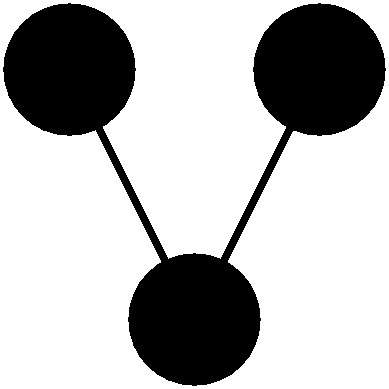
\epsfig{file = ../figures/Vmotif.eps, width=1cm, clip=}      & 13 118 & 14 113 & 14 151 & 15 444 & 2 599 & 0 & 2 510 & 4 200 \\
%   \epsfig{file = ../figures/triangle.eps, width=1cm, clip=}    & 64 & 53 & 55 & 249 & 20 & 8 & 19 & 132 \\
%   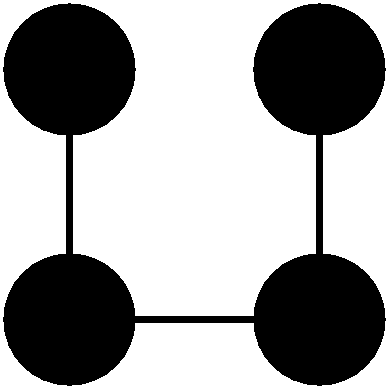
\epsfig{file = ../figures/chainmotif.eps, width=1cm, clip=}  & 90 059 & 84 106 & 85 874 & 176 040 & 26 064 & 3 283 & 23 397 & 78 751 \\
%   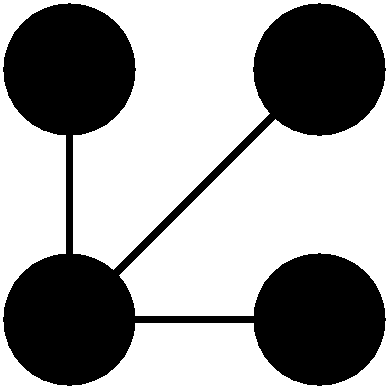
\epsfig{file = ../figures/starmotif.eps, width=1cm, clip=}   & 89 372 & 112 490 & 112 880 & 126 510 & 26 423 & 0 & 36 104 & 58 096 \\
%   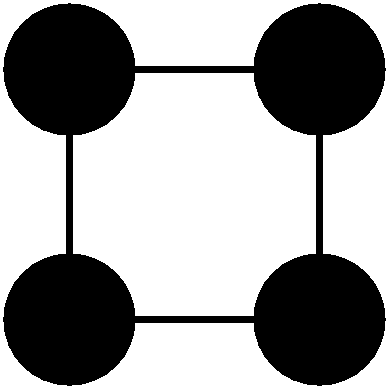
\epsfig{file = ../figures/squaremotif.eps, width=1cm, clip=} & 492 & 285 & 303 & 2 128 & 202 & 27 & 132 & 1 545 \\
%   \epsfig{file = ../figures/whisk.eps, width=1cm, clip=}      & 2 756 & 2 412 & 2 547 & 18 353 & 1 087 & 447 & 1 208 & 13 492 \\
%   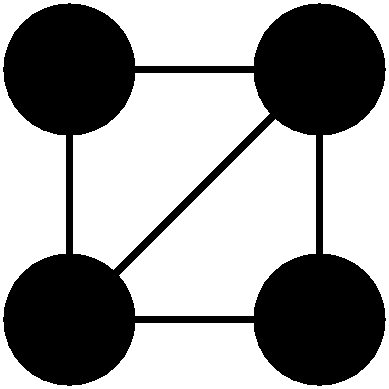
\epsfig{file = ../figures/halfclique.eps, width=1cm, clip=} & 33 & 22 & 25 & 957 & 20 & 10 & 19 & 1 042 \\
%   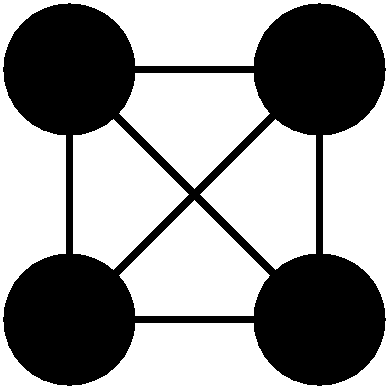
\epsfig{file = ../figures/clique.eps, width=1cm, clip=} & 0 & 0 & 0
%   & 36 & 0 & 0 & 0 & 56 \\
% \end{tabular}
% }
% $$
% Degree distribution fitting is a very strong constraint. \\
% %\\
% The number of occurrences of \emphase{star-like motifs} ('V', hubs,
% {\it etc.})  are \emphase{completely fixed} in the EDF model.


%%%%%%%%%%%%%%%%%%%%%%%%%%%%%%%%%%%%%%%%%%%%%%%%%%%%%%%%%%%%%%%%%%%%%%%%
%%%%%%%%%%%%%%%%%%%%%%%%%%%%%%%%%%%%%%%%%%%%%%%%%%%%%%%%%%%%%%%%%%%%%%%%
%%%%%%%%%%%%%%%%%%%%%%%%%%%%%%%%%%%%%%%%%%%%%%%%%%%%%%%%%%%%%%%%%%%%%%%%
%%%%%%%%%%%%%%%%%%%%%%%%%%%%%%%%%%%%%%%%%%%%%%%%%%%%%%%%%%%%%%%%%%%%%%%%
\end{document}
%%%%%%%%%%%%%%%%%%%%%%%%%%%%%%%%%%%%%%%%%%%%%%%%%%%%%%%%%%%%%%%%%%%%%%%%
%%%%%%%%%%%%%%%%%%%%%%%%%%%%%%%%%%%%%%%%%%%%%%%%%%%%%%%%%%%%%%%%%%%%%%%%
%%%%%%%%%%%%%%%%%%%%%%%%%%%%%%%%%%%%%%%%%%%%%%%%%%%%%%%%%%%%%%%%%%%%%%%%
%%%%%%%%%%%%%%%%%%%%%%%%%%%%%%%%%%%%%%%%%%%%%%%%%%%%%%%%%%%%%%%%%%%%%%%%

